\documentclass{article}

\usepackage{arxiv}

\usepackage[utf8]{inputenc} % allow utf-8 input
\usepackage[T1]{fontenc}    % use 8-bit T1 fonts
\usepackage{lmodern}        % https://github.com/rstudio/rticles/issues/343
\usepackage{hyperref}       % hyperlinks
\usepackage{url}            % simple URL typesetting
\usepackage{booktabs}       % professional-quality tables
\usepackage{amsfonts}       % blackboard math symbols
\usepackage{nicefrac}       % compact symbols for 1/2, etc.
\usepackage{microtype}      % microtypography
\usepackage{graphicx}

\title{Assessing the influence of dopamine and mindfulness on the
formation of routines in visual search}

\author{
    Kelly G. Garner
   \\
    School of Psychology \\
    University of New South Wales \\
  Sydney, NSW \\
  \texttt{\href{mailto:kelly.grace.garner@unsw.edu.au}{\nolinkurl{kelly.grace.garner@unsw.edu.au}}} \\
   \And
    Li-Ann Leow
   \\
    School of Psychology \\
    The University of Queensland \\
  St.~Lucia, QLD \\
  \texttt{} \\
   \And
    Aya Uchida
   \\
    School of Psychology \\
    The University of Queensland \\
  St.~Lucia, QLD \\
  \texttt{} \\
   \And
    Christopher Nolan
   \\
    School of Psychology \\
    The University of New South Wales \\
  Sydney, UNSW \\
  \texttt{} \\
   \And
    Ole Jensen
   \\
    Center for Human Brain Health \\
    University of Birmingham \\
  Birmingham, UK \\
  \texttt{} \\
   \And
    Marta Garrido
   \\
    School of Psychological Sciences \\
    University of Melbourne \\
  Melbourne, VIC \\
  \texttt{} \\
   \And
    Paul E. Dux
   \\
    School of Psychology \\
    The University of Queensland \\
  St.~Lucia, QLD \\
  \texttt{} \\
  }


% tightlist command for lists without linebreak
\providecommand{\tightlist}{%
  \setlength{\itemsep}{0pt}\setlength{\parskip}{0pt}}


% Pandoc citation processing
\newlength{\cslhangindent}
\setlength{\cslhangindent}{1.5em}
\newlength{\csllabelwidth}
\setlength{\csllabelwidth}{3em}
\newlength{\cslentryspacingunit} % times entry-spacing
\setlength{\cslentryspacingunit}{\parskip}
% for Pandoc 2.8 to 2.10.1
\newenvironment{cslreferences}%
  {}%
  {\par}
% For Pandoc 2.11+
\newenvironment{CSLReferences}[2] % #1 hanging-ident, #2 entry spacing
 {% don't indent paragraphs
  \setlength{\parindent}{0pt}
  % turn on hanging indent if param 1 is 1
  \ifodd #1
  \let\oldpar\par
  \def\par{\hangindent=\cslhangindent\oldpar}
  \fi
  % set entry spacing
  \setlength{\parskip}{#2\cslentryspacingunit}
 }%
 {}
\usepackage{calc}
\newcommand{\CSLBlock}[1]{#1\hfill\break}
\newcommand{\CSLLeftMargin}[1]{\parbox[t]{\csllabelwidth}{#1}}
\newcommand{\CSLRightInline}[1]{\parbox[t]{\linewidth - \csllabelwidth}{#1}\break}
\newcommand{\CSLIndent}[1]{\hspace{\cslhangindent}#1}

\begin{document}
\maketitle


\begin{abstract}
Given experience in cluttered but stable visual environments, our
eye-movements adapt to form stereotyped routines that sample the
locations most likely to offer task-relevant information, while not
mixing-up routines between similar task-settings. Both dopamine
signalling and mindfulness have been posited as factors that influence
the formation and deployment of such routines, yet quantification of
their impact remains to be tested in healthy humans. Over two sessions,
participants observed a gaze contingent display comprised of a 4 x 4
grid of doors, and were instructed to fixate on doors to open them to
find hidden targets. Within each session, doors appeared in either one
of two colours, with colour signalling differing likely target
locations. We derived measures for how well participants learned the
target locations (accuracy), how routine was their deployment of
eye-movements (stereotypy), and how much participants mixed-up colour
(task) settings (setting accuracy). Participants received either
levodopa (dopamine precursor) or placebo (vitamin C) across the 2
sessions, administered under double-blind conditions. Dopamine and trait
mindfulness (assessed by questionnaire) interacted to influence both
accuracy and stereotypy. Increasing dopamine improved accuracy and
reduced stereotypy for individuals scoring high for mindfulness, and
induced the opposite pattern for low mindfulness scorers. Dopamine also
disrupted setting-accuracy invariant to mindfulness. Therefore,
mindfulness modulates the impact of dopamine on the accuracy and
stereotypy of eye-movement routines, whereas increasing dopamine
promotes mix-ups between task-settings, regardless of mindfulness. These
findings provide a link between non-human and human models regarding the
influence of dopamine on the formation of task-relevant eye-movement
routines, and provide novel insights into behaviour-trait factors that
modulate the use of experience when building adaptive repertoires.
\end{abstract}

\keywords{
    habit
   \and
    sequence
   \and
    dopamine
   \and
    mindfulness
   \and
    eye-movements
  }

\hypertarget{introduction}{%
\section{Introduction}\label{introduction}}

Given stable environmental contingencies, it is adaptive for an organism
to develop routine ways of performing tasks requiring multiple
responses. Dopamine is assumed to play a key role in the neural
computations that underlie the formation of task routines. A large body
of evidence shows that dopaminergic midbrain neurons encode reward
prediction errors (e.g. Schultz, Apicella, and Ljungberg 1993; Hollerman
and Schultz 1998; Waelti, Dickinson, and Schultz 2001), a teaching
signal that computes the value of actions (Sutton and Barto 2018). A
comparable signal in striatum marks the difference between expected and
actual saccadic sequence lengths used by macaques to attain reward
during visual search (Desrochers et al. 2010; Desrochers, Amemori, and
Graybiel 2015). This signal is assumed to reflect a cost-benefit signal
that computes the value of saccadic routines. There also exists a large
body of evidence from rodent and macaque models suggesting that
increased striatal dopamine availability speeds the transition from
goal-directed to habitual control of behaviour (Harmer and Phillips
1998; Nelson and Killcross 2006; Nadel et al. 2021, 2021), the latter of
which is assumed to govern performance of routines (Dezfouli and
Balleine 2012; Dezfouli, Lingawi, and Balleine 2014; Desrochers,
Amemori, and Graybiel 2015; Graybiel and Grafton 2015; Smith and
Graybiel 2016). Although this evidence implicates dopamine in the
formation of task-relevant routines, whether dopamine availability
modulates the formation of saccadic routines in healthy humans remains
an open question.

One way to address this question is to increase dopamine availability
via administration of levodopa, a precursor to dopamine. levodopa
administration in humans has been associated with increased striatal
activity in response to positive reward prediction errors, assessed
using blood-oxygenation-level-dependent BOLD responses (Pessiglione et
al. 2006), and with reduction of explorative choices during instrumental
learning (Shohamy et al. 2006; Chakroun et al. 2020). This suggests that
levodopa may increase the perceived value of actions by inducing
optimistic evaluations of outcomes (FitzGerald, Dolan, and Friston
2015), possibly by disrupting feedback processing (Shohamy et al. 2006).
Elevating dopamine availability via levodopa may therefore have a
comparable impact on the cost-benefit computations driving the formation
of saccadic routines during visual search. Specifically, levodopa may
promote an optimistic evaluation of the performed sequence, increasing
the probability that it is adopted as a routine.

For task-oriented routines to be adaptive, it is also required that they
are not mixed-up between tasks, despite overlap in the situational cues
and actions that mark task environments. Dopamine is assumed to play a
modulatory role in the activation of task-relevant behaviours in
response to relevant situational cues (Budzillo et al. 2017), as well as
promoting the formation of routines. Patients with Parkinson's Disease
consistently show deficits switching between simple sensorimotor tasks
(Cools et al. 2001; Wiecki and Frank 2010), as do healthy participants
who have been administered D2 antagonists (Mehta et al. 2004). Such
findings have been accounted for by assuming that decreased dopamine
causes increased uncertainty about the probability of being in a
specific task-state (Friston et al. 2012). These assumptions are based
on evidence from constrained tasks - i.e.~when single correct responses
are required for given stimuli. In contrast, saccadic routines are often
formed from a self-selected set of many possible eye-movements, and it
is unclear whether dopamine modulates switching between such routines.
If an impact is observed, it is unclear whether the effect of increasing
dopamine is opposite to that of depleted dopamine, i.e.~does increasing
dopamine availability promote segregation of task routines? Or, does
increasing dopamine availability make it more difficult to switch
between routines, thereby increasing the probability that they will get
mixed up?

A further but less frequently discussed component of the processes
underlying task routine learning and deployment, is the brain's
representation of task-relevant cues and actions. Presumably, the
organism that encodes an accurate representation of cues, actions and
outcomes is at an adaptive advantage when forming and deploying
task-relevant routines. A growing body of empirical evidence suggests
that mindfulness may modulate such representations. Mindfulness has been
defined as a mental state that emphasises current sensory and internal
inputs (Davids 1900; Shapiro et al. 2006), and as such is well-placed to
promote accurate task-representations. In support of this, mindfulness
practice has been associated with increased error monitoring during
cognitively challenging tasks (Andreu et al. 2017), and with greater
sensitivity to dynamics in operant reinforcement contingencies (Chen and
Reed 2023; Reed 2023). This suggests that increased mindfulness is
associated with a task representation that is more sensitive to the
stimulus, response and outcome contingencies that make up the
task-state.

What could be the modulatory influence of mindfulness on the formation
and deployment of task-relevant routines? Mindfulness appears to have
opposing influences to dopamine on routine learning and task-switching:
individuals low in trait mindfulness are faster to exploit sequential
regularities in stimulus-response tasks (Stillman et al. 2014), and
exploitation of such regularities are assumed to support habitual
responses (Dezfouli and Balleine 2012; Dezfouli, Lingawi, and Balleine
2014). Mindfulness may also promote task-switching; higher levels of
trait mindfulness has been associated with decreased reliance on past
behaviours when stimuli are conserved across tasks that carry different
cognitive demands (Greenberg, Reiner, and Meiran 2012; Kuo and Yeh
2015). Indeed both reinforcement learning (RL) and active inference
frameworks have been used to posit that mindfulness and dopamine may
modulate common mechanisms, but may oppose each other in the direction
of their influence. In the case of RL, mindfulness is assumed to
attenuate striatal reward prediction errors (Kirk and Montague 2015;
Kirk et al. 2019), possibly via greater regulation from stronger
cortical representations of subjective values and internal states (Kirk
et al. 2014). In the case of active inference, both dopamine (Friston et
al. 2012; FitzGerald, Dolan, and Friston 2015) and mindfulness
(Laukkonen and Slagter 2021; Giommi et al. 2023) are assumed to modulate
the estimate of uncertainty that is used to weight task-relevant
prediction errors, with mindfulness determining the level of abstraction
where updating is emphasised. These lines of evidence suggest that high
trait mindfulness may negate or enhance the impact of elevated dopamine
on task-relevant routines, yet this relationship remains quantitatively
untested.

Using a novel task designed to test the formation and deployment of
task-relevant saccadic routines in humans, we sought to test whether
administration of levodopa increased suboptimal routine formation, and
whether increased dopamine positively or negatively modulated switching
between routines. We further sought to test whether higher levels of
trait mindfulness offered a buffer against the impacts of increased
dopamine availability. To preview the results, levodopa decreased
accuracy and promoted routine formation in individuals with low
trait-mindfulness, whereas high trait-mindfulness was associated with
the opposite pattern. Regardless of mindfulness, dopamine hampered
switching between routines by increasing mix-ups.

\hypertarget{methods}{%
\section{Methods}\label{methods}}

\label{sec:Methods}

\hypertarget{participants}{%
\subsection{Participants}\label{participants}}

A total of 40 participants (mean age: 24.5, sd: 5, 30 female, 10 male)
were recruited using the undergraduate and paid SONA pools administered
by the University of Queensland. All procedures were cleared by the
University of Queensland Human Research ethics committee
{[}2017/HE000847{]}, and were conducted in accordance with the National
Statement on Ethical Conduct in Human Research. Participants were over
18 years old, had no known neurological and psychiatric conditions
(assessed by self report), and no contraindications to levodopa, as
assessed by the levodopa safety screening questionnaire. Informed
consent was obtained at the start of the first session.

\hypertarget{procedure}{%
\subsection{Procedure}\label{procedure}}

Participants attended two sessions, spaced approximately 1 week apart.
After initial blood pressure and mood assessments (Bond and Lader 1974),
participants received either placebo (vitamin C) or levodopa (Madopar
125: 100 mg levodopa and 25 mg Benserazide Hydrochloride), crushed and
dispersed in orange juice, now referred to as the `placebo' and
`dopamine' sessions respectively. The solution was prepared by an
experimenter who did not administer the remaining experimental
procedures. This protocol was sufficient to achieve double blinding in
previous work (Chowdhury et al. 2012, 2013). Participants then completed
the Five Facet Mindfulness Questionnaire (Baer et al. 2006) and the
Barratt Impulsivity Scale {[}BIS; Patton, Stanford, and Barratt
(1995){]}, as trait impulsivity scores are associated with midbrain
dopamine D2/D3 receptor availability (Buckholtz et al. 2010). Around 30
minutes after drug administration, participants completed a second BP
and mood rating assessment. Participants then completed the practice
stage of the task, so that the experimental stage began approximately 40
minutes after drug ingestion, within the window of peak plasma
availability (\textbf{continPharmacokineticslevodopa2010?}). At the end
of the session, participants completed the final BP and mood rating
assessment and were asked whether they thought they had been given the
active or placebo drug.

\hypertarget{apparatus}{%
\subsection{Apparatus}\label{apparatus}}

The experimental task was run with custom code\footnote{\url{https://github.com/kel-github/variability-decision-making}},
written using Matlab 2012b (32 bit) and Psychtoolbox v3.0.14, on a
Windows 7 (64-bit) on a Dell Precision T1700 desktop computer, displayed
using a ASUS VG248 monitor. Gaze coordinates (x, y) were sampled at 120
Hz using a monitor-mounted iView Red-m infrared eye tracker
(SensoMotoric Instruments GmbH, Teltow, Germany). Participants were
seated from the monitor at an approximate viewing distance of 57 cm, and
positioned on a chin-rest for the duration of the task.

\hypertarget{experimental-task}{%
\subsection{Experimental Task}\label{experimental-task}}

Each trial began with a fixation dot presented centrally on a grey
screen {[}RGB: 200 200 200{]}. Participants were instructed to fixate on
the dot to begin a trial. After 1000 ms of continuous correct fixation
samples (within 100 pixels of fixation), a square was presented that
comprised 18° visual angle along each length. The square could be one of
four possible colours {[}RGBs: 87, 208, 169; 267, 145, 52; 167, 162,
229; 239, 91, 158{]}. After 1000 ms, a 4 x 4 grid of smaller squares
appeared within the larger square, in a darker version of the background
colour ({[}RGB{]}-50). Each square comprised 2.6°. Participants were
instructed that the 4 x 4 grid represented doors, and that they were to
use their eyes to open the doors to find where the target was hiding.
Participants were instructed that they were to fixate on a single door
to open it. When participants had fixated on a door for over 300 ms, the
door either turned black {[}RGB: 50, 50, 50{]}, to denote the absence of
a target, or the target was displayed and the trial was terminated. If
the door had turned black, it returned to its previous colour as soon as
it was detected that the participant had moved their eyes from the door.
Targets were animal images drawn randomly on each trial from a pool of
100 images taken from the internet. The time at which the target was
available to be found varied from trial to trial, with the onset being
drawn from a uniform distribution between 500-2000 ms. Once the target
was available and the correct door selected, the target was displayed
for 750 ms. Upon termination of the trial, the grey screen and white
fixation cross were presented (see Fig \ref{fig:taskfig}A).

In each session, participants saw the display in two possible colours.
Participants were instructed that each colour represented a world, and
that the animals had different places they preferred to hide, depending
on the world they were in. There were four possible target locations
within each world, or from here on, each setting. For each setting, 1
door from each quadrant was selected as one of the 4 possible target
locations (see Fig \ref{fig:taskfig}B), with the constraint that target
locations could not overlap between settings. Thus each colour reflected
a setting in which participants could establish a set of task-relevant
eye-movements, i.e.~towards the 4 possible target locations. Note that
within each setting, the target was equally likely to appear behind any
one of the 4 target doors (p=.25) and would never appear behind the
remaining doors (p=0). Colour-target location mappings were
counterbalanced across participants, as was the assignment of colours to
sessions. Participants completed 80 trials in each setting. Eye-movement
calibration and validation was performed every 20 trials. Participants
were also shown the standard QWERTY keyboard and were instructed that
they could press `x' at any time to perform a new calibration and
validation if they felt that their eye-movements were no longer being
registered accurately.

\begin{figure}

{\centering 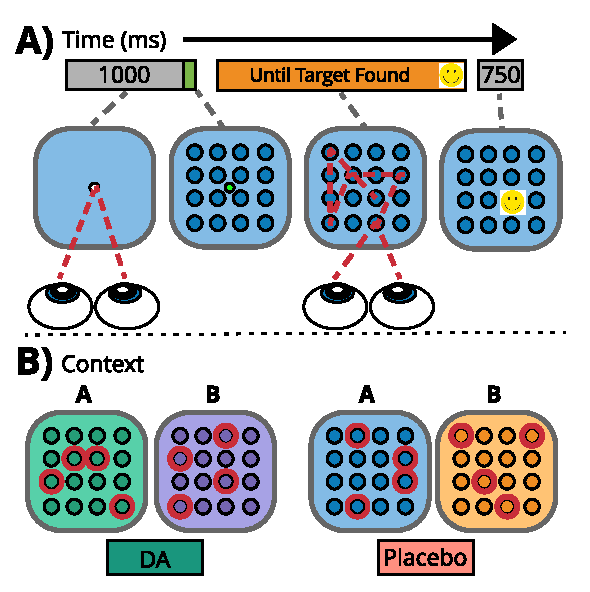
\includegraphics[width=0.7\linewidth]{../../images/DA_ExpTask} 

}

\caption{Experimental Task. A) A single trial where participants use their eyes to open doors to locate a target. B) Contexts and sessions: in each session, participants are exposed to two colour contexts each with 4 unique and equiprobable target locations. Colours and target locations were counterbalanced across participants and sessions. In each session, levodopa (DA) or placebo is administered under double blind conditions.}\label{fig:taskfig}
\end{figure}

\hypertarget{statistical-approach}{%
\subsection{Statistical Approach}\label{statistical-approach}}

The analysis was designed to assess how well participants learned the
target locations, the extent to which participants formed a routine for
door selections (how stereotypical they became in their order of
door-selections), and how well they disambiguated between settings. We
modelled how these elements of performance were modulated by the
dopamine and mindfulness factors. All custom analysis code is available
online\footnote{\url{https://github.com/kel-github/DA_VisRoutes}}. The
analysis was performed using R and RStudio v2022.07.2 (RStudio Team
2020), and can be reproduced in the Neurodesk container environment
(Renton et al. 2022).

\hypertarget{data-cleaning}{%
\subsubsection{Data cleaning}\label{data-cleaning}}

We asserted that a door could not be selected twice consecutively, and
collapsed any consecutive selections into a single selection. As the
final door selection of every trial was fixed (i.e.~finding the target
location ends the trial), we removed the final selection from each trial
for the stereotypy (routine) analysis defined below. We excluded data
from one participant whose total number of door selections was greater
than 3 standard deviations from the mean across both sessions. The
remaining 39 datasets were retained for all of the analyses. Note that
this is more inclusive than our pre-registered plan for data
exclusions\footnote{\url{https://osf.io/2y6pk}}. Based on pilot data, we
had planned to exclude participants who scored \textless{} 65\% accuracy
over the course of a session. Analysis of the final sample suggested
that this was too stringent, as this resulted in the exclusion of 14 of
40 participants. We have not analysed the data with the exclusion of
these participants, owing to the large drop in statistical power for the
individual differences component of the analysis.

\hypertarget{accuracy}{%
\subsection{Accuracy}\label{accuracy}}

We first sought to determine the extent to which levodopa and
mindfulness influenced the learning of target locations (accuracy). Data
was grouped into blocks of 10 trials per setting, and grouped across
settings, resulting in 8 blocks of 20 trials. We computed for each block
the proportion of door selections that were target relevant (TR) given
the current setting (i.e.~the setting presented on trial t). We assessed
the influence of block, drug and mindfulness on accuracy using Bayesian
mixed-model logistic regression. Accuracy was assumed to be drawn from a
binomial distribution (1=target door, 0=non-target door). We then
estimated the probability of drawing a target-door from the total number
of door selections, using a logit link function to convert probabilities
to log-odds. Thus the resulting regression parameter values reflect
changes to the log-odds of accurate door selections.

For this and following analyses, we identified the model that best fit
the data, and made inference over the resulting parameters. We report
the 95\% confidence intervals (CIs) of the parameter posteriors, and
assume a reliable effect when the 95\% CIs do not include zero. Models
were fit using the BRMS (Bürkner 2017) interface for Stan (Team, n.d.)
and RStan (Stan Development Team 2023). We used the default weakly
informative priors as specified in (Bürkner 2017). Specifically, fixed
and random effect \(\beta\) coefficients were given a flat prior,
intercept and standard deviations were assumed to be drawn from a
student's \(t\) distribution (df=1, location=0, scale=2.5), and the
LKJ-correlation prior with parameter \(\zeta\) \textgreater{} 0 was used
for the parameter covariance matrix. For each model, we checked for
parameter recovery using simulated data. Once fitted, we checked that
the residuals showed no signs of systematic error, that the chains had
converged, and that \(\hat{R}\) values were less than 1.01.

To eschew an overly large model space, and in line with our
pre-registration, we first fit models that contained each possible
combination of the block and drug regressors (and associated random
effects), and found the best model using leave-one-out (LOO) cross
validation, as implemented in Vehtari et al, (2017). Rather than
re-fitting the model for every sub-sample, which is computationally
expensive, this algorithm instead computes analytically how the
predictions made by the model are influenced by each data point. The
relationship between this influence and the change in the posterior that
would occur as a consequence of holding out each data point can be used
to compute the expected log-pointwise predictive density (ELPD). This
quantifies the error that would occur in the prediction of each data
point, when that data point is withheld from the model fitting
procedure. The resulting ELPDs are then compared between models. We
report the ELPD difference between the winning model and the next best
models (a negative value indicates preference for the winning model). As
the ELPD is computed using each observed data point, it is possible to
estimate the standard error (SE) of the difference between models
(Vehtari et al, -Vehtari, Gelman, and Gabry (2017)). We therefore also
report the ratio of the ELPD difference to the SE, as this provides a
proxy for statistical significant differences between models. (Note that
in the pre-registration document we had proposed to compare models using
the deviance information criterion (DIC). As LOO is more robust than DIC
to influential observations, and is readily implemented for use with
BRMS model objects, we opted to use LOO instead of DIC).

Upon identifying the best model, we then added the mindfulness
regressor, fitting all possible combinations, and once again selected
the best model. Last we controlled for trait impulsivity by adding BIS
scores as a main effect to the winning model. Note that in no cases did
adding BIS scores improve the model. The full set of model comparisons
are presented in the supplementary materials.

\hypertarget{setting-accuracy}{%
\subsection{Setting Accuracy}\label{setting-accuracy}}

We next sought to model the impact of levodopa and mindfulness on task
mix-ups. To measure the extent of task mixing, we computed a measure of
setting-accuracy. This measure indexes the total number of door
selections (n) that were appropriate for the colour setting displayed on
trial t (current setting, CS), relative to the number of door selections
that were appropriate for the setting not displayed on trial t (i.e.~the
other-setting from that session, OS):

\[
setting\mathrm{-}acc = \frac{\sum{CS_{n}}}{\sum{(CS_{n}, OS_{n})}}
\]

We modelled the influence of levodopa and mindfulness on
setting-accuracy using the Bayesian mixed-effects logistic regression
approach described above (Note that in the pre-registration document we
had suggested to include a regressor for context. Visual inspection of
the data showed that setting-accuracy was highly comparable across
contexts {[}see Supplemental Figure 2{]}. We therefore opted to simplify
the model space and collapse over this factor).

\hypertarget{stereotypical-door-selections}{%
\subsection{Stereotypical door
selections}\label{stereotypical-door-selections}}

Next, we determined the extent to which door-selections became routine
over the course of the task - specifically, how much the order of door
selections increased in stereotypy, and whether dopamine and mindfulness
modulates the extent of stereotypy. Here we use stereotypy as a proxy
for routine formation, and we define stereotypy as the tendency to
choose doors in the same order, over trials (e.g. Desrochers, Amemori,
and Graybiel 2015).

In order to index stereotypy, we reasoned that stereotypy should result
in an increase in the probability of a subset of door transitions. This
stands in contrast to when making door selections in an exploratory, or
non-stereotyped way, where there should be an even representation of
door transition probabilities. Therefore, the transition probability
matrices of individuals engaged in more stereotypical door selections
should show higher variance than those who are not engaging in
stereotypical door selections. We computed trial level transition
probability matrices, and calculated the variance of each matrix.
Variances were then collapsed across settings and trials to form a
stereotypy score for each participant, session and block.

The resulting stereotypy scores were subject to a comparable Bayesian
mixture modelling approach as described above with a few key
differences; the stereotypy scores were assumed to be drawn from a
skewed normal distribution \(\mathcal{N}(\mu, \sigma, \alpha)\) whose
mean (\(\mu\)) was defined by the regression parameters (the
distribution of stereotypy scores are presented in Supplemental Figure
3). \(\sigma\) was assumed to be drawn from a Student's t distribution
(df=3, location=0, scale=2.5), the skew parameter (\(\alpha\)) was
assumed to be drawn from a normal distribution \(\mathcal{N}(0,4)\). The
remaining priors for the intercept, beta-coefficients and parameter
covariance matrix were defined in the same manner as for the accuracy
data models. As the log-log plot of variances vs block suggested a power
function, analysis was performed on the logged data. This ensured that
the relationship between block and variance values was best described by
a straight line. Identification of the winning model proceeded as
described for the accuracy data above.

\hypertarget{blinding-analyses}{%
\subsection{Blinding analyses}\label{blinding-analyses}}

To determine whether awareness of the dopamine intervention could have
contributed to the findings, the probability of participant ratings were
compared to the expected values assuming chance guessing, using a Chi
Square test. BP and mood ratings were each subject to a session
(dopamine vs placebo) x timepoint (pre-drug, pre-experiment,
post-experiment) Bayesian repeated measures ANOVA, implemented using the
BayesFactor package for R (Morey, Rouder, and Jamil 2015) using the
default priors (Rouder et al. 2012).

\hypertarget{results}{%
\section{Results}\label{results}}

Overall, mindfulness and dopamine interacted to show opposing effects on
accuracy and stereotypy, whereas only dopamine modulated setting
accuracy.

\hypertarget{accuracy-1}{%
\subsection{Accuracy}\label{accuracy-1}}

\hypertarget{model-selection}{%
\subsubsection{Model selection}\label{model-selection}}

First we sought the best model in order to make subsequent inference
over the parameters. The model that best accounted for the experimental
factors contained main fixed effects of block and drug, and random
effects for block and drug. Although this model was only closely
preferred to the next most complex model that contained a block x drug
interaction (ELPD diff = -0.33, ELPD:SE = -0.57), it was strongly
preferred to all other models (min ELPD diff = -958.53, ELPD:SE =
-8.65). Adding mindfulness scores improved the predictive accuracy of
the model; the winning model contained an additional main effect of
mindfulness, as well as block x mindfulness and drug x mindfulness
interactions (ELPD diff to best model without mindfulness = -3.12,
ELPD:SE = -0.62). Adding BIS scores did not improve the predictive value
of the model (ELPD diff = -1.95, ELPD:SE = -3.77). Note that although we
draw inferences over parameters from the winning model, our inferences
are the same as if we had used the more complex model that includes the
BIS scores.

\hypertarget{the-effect-of-dopamine-and-mindfulness-on-accuracy}{%
\subsubsection{The effect of dopamine and mindfulness on
accuracy}\label{the-effect-of-dopamine-and-mindfulness-on-accuracy}}

Having established the best model to account for the data, we next
determine the influence of dopamine and mindfulness on accuracy by
making inference over the resulting parameters. Accuracy data plotted by
block x drug session (dopamine vs placebo) are shown in Fig
\ref{fig:accfig}A. Critically, the influence of drug on accuracy was
impacted by mindfulness scores. The drug x mindfulness parameter
differed reliably from zero (mean log odds = -0.12, 95\% CI{[}-0.16,
-0.07{]}, see Fig \ref{fig:accfig}E). To better understand this
interaction, we computed a score for each participant that reflected the
mean accuracy change due to the drug session (\(\mu\) acc{[}dopamine -
placebo{]}). Note that a positive score indicates that performance was
better in the dopamine session relative to placebo. Next we examined the
relationship between dopamine-induced accuracy changes and mindfulness
scores. As can be seen in Fig \ref{fig:accfig}B, there was a positive
relationship between dopamine-induced accuracy changes and mindfulness;
participants scoring higher for mindfulness showed higher accuracy in
the dopamine relative to the placebo session, for example, those scoring
in the highest quartile showed mean accuracy scores of 0.47
(95\%CI{[}0.44, 0.50{]}) during the dopamine session, relative to mean
accuracy scores of 0.41 (95\% CI{[}0.38, 0.43{]}) during the placebo
session. Individuals scoring low on mindfulness numerically showed the
opposite pattern (dopamine mean accuracy = 0.43, 95\% CI{[}0.41,
0.45{]}, placebo mean accuracy = 0.44, 95\%CI{[}0.43, 0.46{]}), note
that Fig \ref{fig:accfig}B shows the difference between these accuracy
scores). Thus the impact of dopamine on the establishment of
task-relevant eye-movements is dependent on the mindfulness state of the
individual.

Participants learned the target door locations over the course of the
sessions, accuracy reliably increased over blocks. Mean accuracy in
block 1 was 0.34 (95\% CI{[}0.32, 0.37{]}), relative to a block 8 mean
of 0.50 (95\% CI{[}0.48, 0.53{]}). The model showed that accuracy
increased by block with an average log odds of = 0.15, (95\% CI{[}0.09,
0.22, Fig \ref{fig:accfig}C). There was also the suggestion of a main
effect of dopamine (mean log odds = 0.04, 95\% CI{[}-0.002, 0.09, Fig
\ref{fig:accfig}D), however, the impact of dopamine on accuracy is
presumably better explained by the drug x mindfulness interaction.

\begin{figure}

{\centering 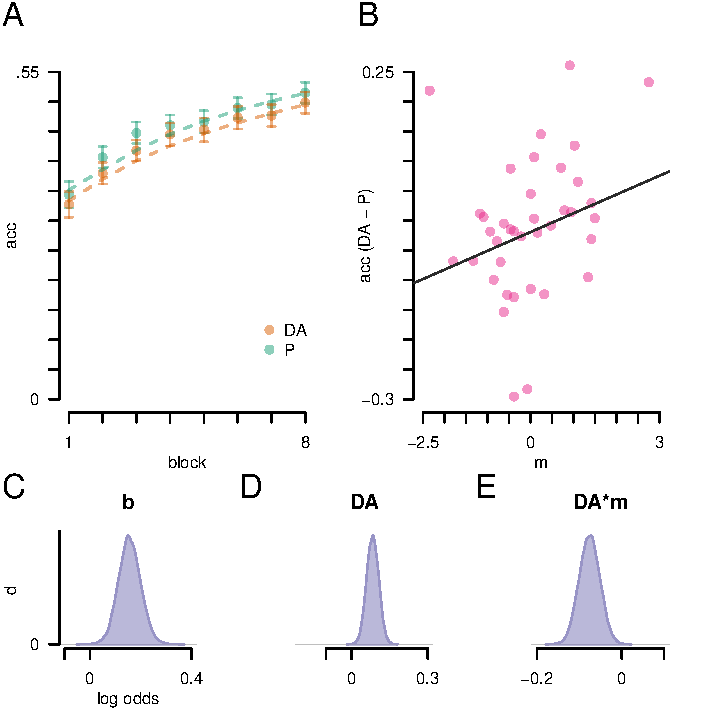
\includegraphics[width=0.7\linewidth]{../../images/acc_fig} 

}

\caption{The influence of dopamine and mindfulness on accuracy. A) Accuracy (acc) data by block and drug. Circles reflect observed average accuracy, dotted lines reflect the fit of the winning model. B) The association between trait mindfulness (x-axis) and the impact of drug on accuracy [dopamine-placebo]. The bottom row shows posterior densities (in log odds) estimated for C) the main effect of block (b), D) the main effect of dopamine, and E) the drug x mindfulness (m) interaction. DA = dopamine, P = placebo, d = density. Error bars reflect within-subject standard error of the mean [SE].}\label{fig:accfig}
\end{figure}

\hypertarget{setting-accuracy-1}{%
\subsection{Setting-Accuracy}\label{setting-accuracy-1}}

\hypertarget{model-selection-1}{%
\subsubsection{Model selection}\label{model-selection-1}}

The best model contained main fixed effects of block and drug, and
random effects for block x drug. Although this model was only closely
preferred to the next most complex model that contained a block x drug
interaction (ELPD diff = -0.66, ELPD:SE = -1.67), it was strongly
preferred to all other models (min ELPD diff = -553.79, ELPD:SE =
-8.35). Adding mindfulness scores improved the predictive accuracy of
the model; the winning model contained an additional main effect of
mindfulness (ELPD diff = -0.13, ELPD:SE = -0.12). Adding BIS scores did
not improve the predictive value of the model (ELPD diff = -0.02,
ELPD:SE = -0.03). Note that although we draw inferences over parameters
from the winning model, our inferences are the same as if we had used
the more complex model that includes the BIS scores.

\hypertarget{drug-and-not-mindfulness-impacts-setting-accuracy}{%
\subsubsection{Drug, and not mindfulness, impacts
setting-accuracy}\label{drug-and-not-mindfulness-impacts-setting-accuracy}}

We next determined the influence of dopamine and mindfulness on
setting-accuracy by making inference over the resulting model parameters
(see Fig \ref{fig:caccfig}). Dopamine reduced setting accuracy; accuracy
was on average 0.64 (95\% CI {[}0.63, 0.65{]}) for the dopamine session,
and 0.66 (95\% CI {[}0.65, 0.68{]}) for the placebo session. The
log-odds of selecting a target door that was specific to the current
setting increased by a mean log odds of 0.07 (95\% CI{[}0.01, 0.13, Fig
\ref{fig:caccfig}A\&B) for the placebo session, relative to the dopamine
session. This suggests that dopamine caused mix-ups between settings.

Setting-accuracy improved over the course of each session; mean accuracy
in block 1 was 0.59 (95\% CI{[}0.58, 0.61{]}), relative to block 8
(mean: 0.69, 95\% CI{[}0.67, 0.71{]}). The model showed that
setting-accuracy increased by a mean log odds of 0.13 (95\% CI{[}0.07,
0.19) over each block (Fig \ref{fig:caccfig}C). In contrast to the
overall accuracy data, mindfulness did show a reliable impact on
setting-accuracy (mean log odds = 0.04, 95\% CI{[}-0.04, 0.13{]}).

\begin{figure}

{\centering 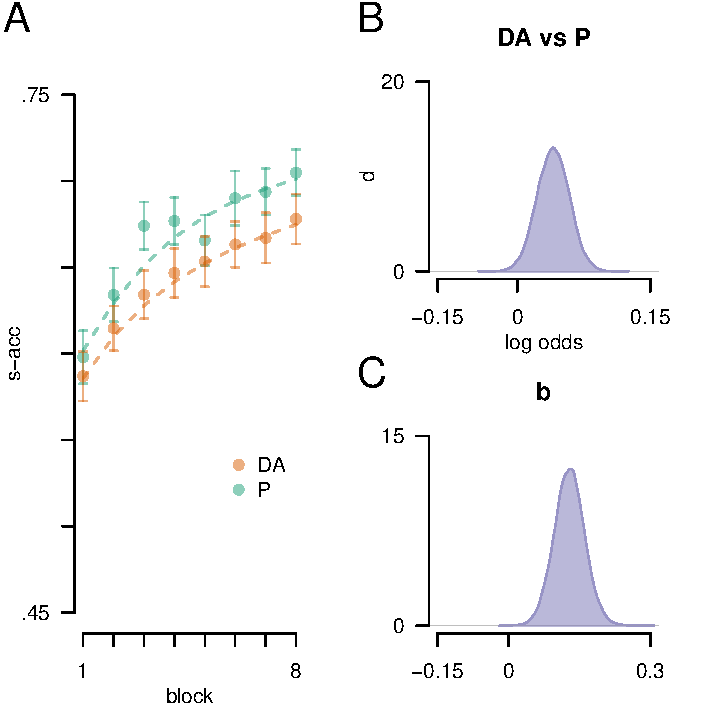
\includegraphics[width=0.7\linewidth]{../../images/cacc_fig} 

}

\caption{The influence of dopamine and mindfulness on setting accuracy. A) Accuracy (acc) data by block and drug. Circles reflect observed average accuracy, dotted lines show the fit of the winning model. B) Estimated posterior density (in log odds) for the main effect of drug (dopamine vs placebo), D) same as in B, but for the main effect of block. DA = dopamine, P = placebo, b = block, d = density. Error bars reflect within-subject standard error of the mean [SE].}\label{fig:caccfig}
\end{figure}

\hypertarget{setting-accuracy-control-analysis}{%
\paragraph{Setting-accuracy control
analysis}\label{setting-accuracy-control-analysis}}

Dopamine influences setting-accuracy, which indexes the likelihood of
door selections that are relevant for the current-setting, relative to
door selections that are relevant for the other-setting. As we exclude
door selections for locations that are never target relevant from the
computation of setting accuracy, it is important to verify that
setting-accuracy scores do indeed reflect mix-ups between settings,
rather than a general task learning deficit. To address this in an
exploratory analysis, we reasoned that if setting-accuracy scores
reflected a general deficit, then `error' door selections should be
drawn randomly from not-target doors (other-setting = 4 \& neither = 8).
A general deficit interpretation suggests that other-setting selections
should be drawn from the total set (other-setting + neither) with \(p\)
= \(\overline{.333}\). If setting-accuracy scores do reflect the
presence of mix-ups, then it would be likely that this error would be
more common than a random door selection, therefore other-setting
selections should occur at levels higher than chance. To test this, we
computed for each participant the probability of other-setting
selections, given the set of other-setting and neither door selections
(\(p_{os}\)), and performed a one-sided t-test, against a null value of
\(p\) = .333. (Note that we opted to use an NHST approach as we had a
point null hypothesis). The \(p_{os}\) data was unlikely under the null
hypothesis (mean = 0.37, 95\% CI{[}0.35, 0.39{]}, \(t\)(38) = 3.62,
\(p\) = 0.0004. Therefore, we reject the hypothesis that the the
dopamine induced drop in setting-accuracy reflects a general learning
deficit.

\hypertarget{stereotypy-of-door-selections-routine}{%
\subsection{Stereotypy of door selections
(routine)}\label{stereotypy-of-door-selections-routine}}

\hypertarget{model-selection-2}{%
\subsubsection{Model selection}\label{model-selection-2}}

The model that best accounted for the stereotypy data contained main
fixed effects of block and drug, and random effects for block x drug.
Although this model was only closely preferred to the next most complex
model that contained a block x drug interaction (ELPD diff = -0.26,
ELPD:SE = -1.29), it was strongly preferred to all other models (min
ELPD diff = -130.14, ELPD:SE = -7.71). Adding mindfulness scores
improved the predictive accuracy of the model; the winning model
contained an additional main effect of mindfulness and a drug x
mindfulness interaction (ELPD diff = -3.15, ELPD:SE = -0.92). Adding BIS
scores did not improve the predictive accuracy of the model (ELPD diff =
-0.54, ELPD:SE = -1.41). Note that although we draw inferences over
parameters from the winning model, our inferences are the same as if we
had used the more complex model that includes the BIS scores.

\hypertarget{the-impact-of-drug-and-mindfulness-on-stereotypy}{%
\subsubsection{The impact of drug and mindfulness on
stereotypy}\label{the-impact-of-drug-and-mindfulness-on-stereotypy}}

Mindfulness and dopamine interacted to impact stereotypy; we observed a
reliable drug x mindfulness interaction (mean \(\beta\) = 0.11, 95\%
CI{[}0.02, 0.21, Fig \ref{fig:stereofig}). Mindfulness scores modulated
the stereotypy difference between the dopamine and placebo sessions; for
example, those scoring in the highest quartile showed mean log variance
scores of -8.74 (95\%CI{[}-8.80, -8.68{]}) during the dopamine session,
relative to mean log variance scores of -8.68 (95\% CI{[}-8.74,
-8.62{]}) during the placebo session. Individuals scoring low on
mindfulness (lowest quartile) showed the opposite pattern (dopamine mean
accuracy = -8.69, 95\% CI{[}-8.75, -8.63{]}, placebo mean accuracy =
-8.72, 95\%CI{[}-8.78, -8.66{]}). To visualise this interaction, we
computed a mean variance change score between drug sessions for each
participant (\(\mu\) stereotypy{[}dopamine - placebo{]}). Note that a
positive score indicates that performance was more stereotyped in the
dopamine session relative to placebo. As can be seen in Fig
\ref{fig:stereofig}B, there was a negative relationship between
drug-induced stereotypy changes and mindfulness. Thus the impact of
dopamine on the formation of eye-movement routines is dependent on the
mindfulness state of the individual.

Participants developed routines over the course of the experiment, as
evidenced by a reliable increase in stereotypy over blocks (mean
increase per block: \(\beta\) = 0.32, 95\% CI{[}0.20, 0.43, Fig
\ref{fig:stereofig}C). In line with the interaction of drug x
mindfulness reported above, the main effect of mindfulness suggested a
negative relationship with stereotypy (mindfulness mean \(\beta\) =
-0.15, 95\% CI{[}-0.26, -0.05, Fig \ref{fig:stereofig}D). Overall,
higher mindfulness scores predicted less stereotypy in door-selection
patterns relative to low mindfulness scores.

\begin{figure}

{\centering 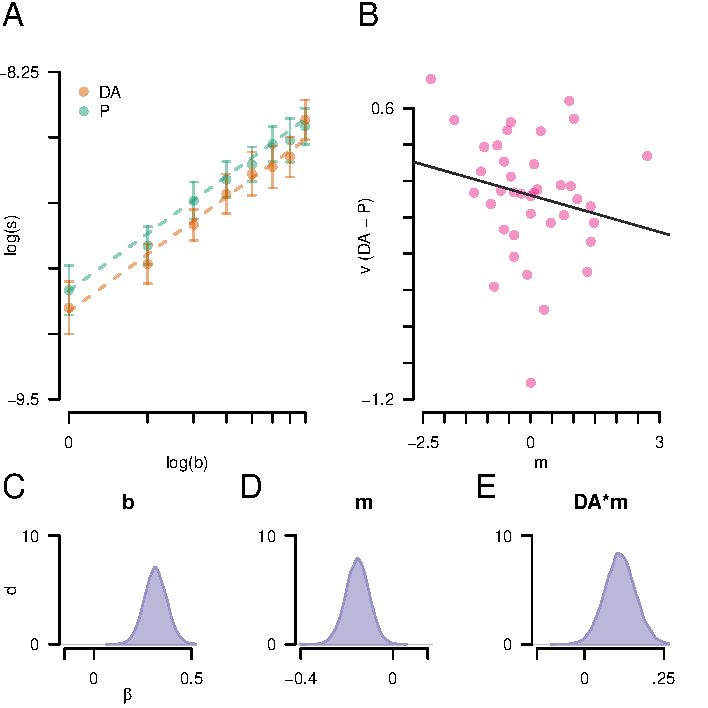
\includegraphics[width=0.7\linewidth]{../../images/s_fig} 

}

\caption{The influence of dopamine and mindfulness on door selection stereotypy. A) Accuracy (acc) data by block and drug. Circles reflect observed average variance (of the transition matrices), dotted lines show the fit of the winning model. B) The association between trait mindfulness (x-axis) and the impact of drug on variance [DA-P]. The bottom row shows posterior densities (in log odds) estimated for C) the main effect of block (b), D) the main effect of dopamine, and E) the drug x mindfulness (m) interaction. DA = dopamine, P = placebo, d = density. Error bars reflect within-subject standard error of the mean [SE].}\label{fig:stereofig}
\end{figure}

\hypertarget{on-the-relationship-between-accuracy-and-stereotypy}{%
\paragraph{On the relationship between accuracy and
stereotypy}\label{on-the-relationship-between-accuracy-and-stereotypy}}

Accuracy and stereotypy showed opposing relationships with mindfulness
and dopamine. Higher mindfulness scores were associated with
dopamine-induced accuracy increases, and stereotypy decreases, relative
to placebo. Individuals scoring low on mindfulness showed a deleterious
influence of dopamine on accuracy, coupled with increased stereotypy,
relative to placebo. As accuracy and stereotypy are possibly, but not
necessarily related, we next sought to ensure that the observed
influences of dopamine and mindfulness on stereotypy was not driven by
accuracy, in an exploratory analyses. We reasoned that such a pattern of
results could be observed if the measures of accuracy and stereotypy
reflected a direct trade off; i.e.~as accuracy goes up, stereotypy goes
down. A correlation analysis ruled out this possibility. We computed
mean accuracy and stereotypy scores for each participant, collapsing
across all experimental factors, and found that accuracy and stereotypy
were positively related (\(r\)(37) = 0.81, \(p\) = 3.51e-10).

Next, to rule out the contribution of accuracy to the stereotypy
results, we added mean accuracy, computed for each block and drug
condition, as a regressor to the winning model. Adding accuracy as a
regressor both clearly improved the predictive accuracy of the model
(ELPD diff = -110.26, ELPD:SE = -6.12), and served to increase certainty
in the interactive influence of mindfulness x drug on stereotypy.
Specifically, the estimated influence of the interaction increased from
\(\beta\) = 0.11 to \(\beta\) = 0.22 (95\% CI{[}0.14, 0.29{]}). Note
that the pattern of remaining results were also consistent between the
two models. Therefore, the data support the notion that mindfulness and
dopamine interact to differently influence accuracy and stereotypy when
participants perform task-relevant saccadic routines.

\hypertarget{blinding-check}{%
\subsection{Blinding check}\label{blinding-check}}

Next we checked if participants knew whether they had received levodopa
or placebo across the two sessions. Participants were asked to report at
the end of each session whether they thought they had received levodopa
or placebo. Participant responses were coded as either correct for both
sessions (cc: observed N = 7), correct for one session and incorrect for
the other (ci: N = 11), or incorrect for both sessions (ii: N = 8). The
probability of the observed guesses was not statistically unlikely given
the null distribution of chance performance (the null hypothesis
specified \(p\)= .25, .5, .25 for cc, ci, ii respectively, \(\chi^2\)(2,
26) = 0.69, \(p\) =0.71). Note that we were unable to include all the
participants in this analysis owing to missing data. Specifically, due
to a miscommunication in the research team, the blinding check questions
contained `Don't know' as a possible response, for which we are unable
to generate a null hypothesis. We therefore only include participants
who made a guess using the levodopa and placebo options across both
sessions.

\hypertarget{mood-and-blood-pressure}{%
\subsection{Mood and blood pressure}\label{mood-and-blood-pressure}}

We also sought to determine whether dopamine influenced physiological
factors such as mood and blood pressure. For mood, the winning model
contained a main effect of time-point and no other fixed effects. This
model was preferred relative to next best model, which contained an
additional main effect of drug (BF = 3.76, ±2.14\%) and was
substantially preferred over the null random intercept model (BF =
514549 ±1.23\%).

Mean blood pressure was computed using the formula: Mean BVP = diastolic
blood pressure (DBP) + 1/3 {[}systolic blood pressure (SBP) -- DBP{]}.
For mean BVP, the winning model contained main effects of both
time-point and drug. This model was barely preferred to the next best
model which contained a time-point x drug interaction (BF = 1.7
±5.69\%), but was strongly preferred to the random intercept model (BF =
5011975 ±3.76\%). Overall, mean BVP was lower in the levodopa session
(mean = 2.181.511261, 95\% CI{[}80.3, 82.8{]}), relative to placebo
(mean = 84.5, 95\% CI{[}83.5, 2.185.504042{]}).

\hypertarget{discussion}{%
\section{Discussion}\label{discussion}}

We investigated the impact of levodopa administration and trait
mindfulness on the learning of task-relevant behaviour sets, and on the
routine nature of their deployment. Participants opened doors to search
for targets in a gaze-contingent display. The colour of the display
signalled likely target locations, making some locations relevant for
only that colour. We assessed how well participants learned target
locations (accuracy), how routine was the order of door selections
across trials (stereotypy), and how well participants learned to
segregate task-routines (setting-accuracy). levodopa impacted accuracy,
stereotypy and setting-accuracy, but in the case of the former two, this
impact was modulated by trait mindfulness. High trait mindfulness
corresponded to increased accuracy and decreased stereotypy, for
levodopa relative to placebo, whereas low trait mindfulness was
associated with the opposite pattern. These results quantify, for the
first time, that increasing systemic dopamine availability induces a
trade-off between accuracy and stereotypy that is modulated by
trait-mindfulness, and that increased dopamine availability increases
routine confusion. These findings carry implications for our theoretical
understanding of how the brain establishes and switches between
task-relevant behavioural routines, which we outline below.

The current findings offer insight into the relationship between
dopamine and mindfulness. Dopamine and mindfulness have been indirectly
related in both the RL (Kirk et al. 2014, 2019) and active inference
frameworks (Friston et al. 2012; FitzGerald, Dolan, and Friston 2015;
Laukkonen and Slagter 2021; Giommi et al. 2023), yet there exists no
other study to-date that assesses their joint impact on behaviour. Here
we find that levodopa and mindfulness jointly modulate learning and
stereotypy, with levodopa yielding conditions of decreased accuracy and
increased stereotypy in low trait mindfulness scorers. We hypothesise
that low mindfulness results in poorer sensory-action representations
which renders the individual more susceptible to error when estimating
the reward value of actions, which is compounded by over-optimistic
estimations induced by elevated dopamine availability. The result is a
failure to differentiate between the actions that do and do not lead to
reward, and an increased probability of reliance on past behaviours.
This could be manifest via impoverished top-down, cortical regulation of
positive prediction errors in striatum (Kirk et al. 2014), as has been
predicted within an RL framework. The same result could also be
accounted for by a decrease in certainty regarding sensory prediction
errors occurring with low mindfulness (Laukkonen and Slagter 2021;
Giommi et al. 2023), in tandem with dopamine inducing inflated certainty
regarding reward outcomes (FitzGerald, Dolan, and Friston 2015), as has
been suggested via the active inference framework.

Note that the two accounts predict comparable outcomes so we are unable
to differentiate between them with the current data. However, the
current findings do constrain these accounts regarding the extent of
overlap between the actions of dopamine availability and mindfulness.
Increased dopamine availability increased routine confusion, regardless
of trait mindfulness. Therefore, there are limitations to the modulatory
influence of mindfulness on the actions of dopamine. The establishment
and maintenance of a task-set is assumed to reflect a superordinate
representation of a goal and the set of actions required to attain that
goal (Schumacher and Hazeltine 2016; Desrochers et al. 2016; Sutton and
Barto 2018; Vaidya et al. 2021; Lee, Hazeltine, and Jiang 2022). The
current data suggest that while dopamine and trait mindfulness can
jointly modulate the learning and execution of subordinate
representations, i.e.~the set of actions used, mindfulness does not
modulate the impact of dopamine on superordinate task representations,
at least under the current task conditions. Future work should determine
whether these observed limits in the modulatory influence of mindfulness
are due to a limited locus of effect, or are due to increased
vulnerability to the impacts of dopamine at superordinate levels of
representation.

The finding that levodopa increased mix-ups between settings extends
previous work showing that dopamine impacts switching between simple
sensorimotor tasks that require only one response (Cools et al. 2001;
Mehta et al. 2004; Wiecki and Frank 2010). Collectively, these findings
point to a U-shaped function linking dopamine levels and task-switching
impairments, in that depleted and inflated levels of dopamine result in
greater task-switching deficits. This observation informs theoretical
accounts of the relationship between dopamine and an agent's ability to
infer the current task state, which have previously only considered the
impacts of depleted dopamine (Friston et al. 2012). However, as the
currently studied behaviours are more complex than the constrained
sensorimotor tasks that are typically used in task-switching studies,
future work should verify whether levodopa administration comparably
impacts task-switching in simple sensorimotor tasks, and whether
depleted dopamine impacts switching between tasks requiring multiple
responses. This will determine whether the relationship between dopamine
and task-switching is comparable across tasks or is task dependent.

To minimise setting mix-ups, an agent must maintain a representation of
the actions required to achieve the task goal, and must associate this
representation to the correct task cues. We found that levodopa
consistently increased the probability that actions from a non-relevant
task-set would be selected during current task performance, whereas the
probability that an erroneous action was selected varied across
individuals according to their trait mindfulness. Therefore, the most
consistent locus of task-set confusion is between actions that have been
credited as successful in either task-context. What remains to be
determined is whether levodopa caused task-interference, or attenuated
the ability to associate successful actions with the appropriate
situational cues. If the latter is true, then levodopa would have caused
individuals to learn one task, that did not incorporate the colour cue
as a relevant disambiguating signal. We seek to arbitrate between these
possibilities in future work.

In contrast to expectations, levodopa lead to an overall reduction in
stereotypy in door selections, suggesting that increased dopamine
availability reduces the probability of forming a routine when
performing multiple responses. This is in contrast to previous findings
showing that increased dopamine speeds the transition to habit formation
(Harmer and Phillips 1998; Nelson and Killcross 2006; Nadel et al. 2021,
2021). As with task-switching studies, such findings are largely based
on rodent models using tasks comprising one or two stimulus-response
associations. Our findings show that in the case of sets of
task-relevant saccades, increasing dopamine does not necessarily lead to
increased habit formation. Moreover, levodopa did not improve accuracy
overall, suggesting that our results cannot be solely attributed to
levodopa increasing model-based control (Wunderlich, Smittenaar, and
Dolan 2012; Kroemer et al. 2019; Deserno et al. 2021), or adjusting the
balance between exploitation and exploration (Kayser et al. 2015;
Chakroun et al. 2020).

What then is the influence of dopamine on the cost/benefit computations
that drive routine formation? In accordance with previous work with
non-human primates (Desrochers et al. 2010; Desrochers, Amemori, and
Graybiel 2015), the current data do suggest that dopamine is a modulator
of the computations that drive routines in humans. However, the current
data also show that the modulatory influence of dopamine is dependent on
the behaviour-trait state of the individual. Specifically, increased
dopamine appears to drive individuals low in mindfulness towards a
stereotypical solution that is suboptimal in terms of accuracy,
suggesting a poor evaluation of sequence costs relative to benefits. In
contrast, individuals high in trait mindfulness show increased accuracy
but reduced stereotypy, suggesting an appropriate crediting of
successful actions, but also suggesting some volatility in their
execution. While the current data demonstrate the applicability of
dopamine signalling to the computations that underlie the formation of
routines, the data also show further work is required to determine the
internal state variables that determine whether increased dopamine
availability will have a positive or negative impact on performance.

The current work is not without limitations. A difference was found in
mean BVP between the levodopa and placebo sessions, suggesting more
general physiological differences between the sessions. However, the
effect of levodopa on blood-pressure is well characterised, and depends
partly on the effective dose (dose per kilogram,
\textbf{goldbergCardiovascularEffectslevodopa1971?}). It is unlikely
that low and high mindfulness individuals differed systematically in
terms of effective dose. Participants were also not able to detect
whether they had received levodopa or placebo above what would be
expected by chance. Therefore, the physiological changes appeared to not
be subjectively detectable, lowering the likelihood that discernible
subjective differences impacted the results. Note that although the
power of our blinding test was lowered owing to missing data, the
remaining N was comparable to sample sizes from previous investigations
into the impact of dopaminergic pharmacological intervention on
decision-making, that employed comparable blinding tests (Leow et al.
2023; Pine et al. 2010; Wunderlich, Smittenaar, and Dolan 2012;
\textbf{volevodopaImpairsProbabilistic2016?}; Vo, Seergobin, and
MacDonald 2018).

Although accuracy and stereotypy theoretically need not be correlated,
we did find a moderate positive correlation between the two measures.
Critically, the modulatory influence of mindfulness and dopamine on
stereotypy was found to be larger after accounting for accuracy.
Furthermore, accuracy and stereotypy were at antithesis to each other
with regard to the demonstrated impacts of mindfulness and levodopa.
Nonetheless, further work should be done to confirm the dissociable
impact of dopamine and mindfulness on these two aspects of performance.
We shall seek to achieve this in future studies by controlling task
parameters to maintain accuracy, while examining modulations to
stereotypy.

We sought to determine the modulatory influence of dopamine availability
and trait-mindfulness on the formation and deployment of task-relevant
saccadic routines. We found evidence for theoretical assertions that
dopamine and mindfulness share overlap in their locus of influence, but
also demonstrated boundaries in that overlap. Mindfulness modulated the
impact of dopamine on task-learning and routine development, with
levodopa administration resulting in low mindfulness individuals being
more likely to show impaired learning and increased stereotypy.
Invariant to trait-mindfulness, levodopa increased the likelihood of
mix-ups between task settings, suggesting that dopamine either hampers
the binding of actions to situational cues, or promotes confusion
between task-states. Collectively, these data suggest that the fidelity
of situational representations interact with reinforcement learning
systems to drive the formation of behavioural routines.

\hypertarget{references}{%
\section*{References}\label{references}}
\addcontentsline{toc}{section}{References}

\hypertarget{refs}{}
\begin{CSLReferences}{1}{0}
\leavevmode\vadjust pre{\hypertarget{ref-andreuBehavioralElectrophysiologicalEvidence2017}{}}%
Andreu, Catherine I., Cristóbal Moënne-Loccoz, Vladimir López, Heleen A.
Slagter, Ingmar H. A. Franken, and Diego Cosmelli. 2017. {``Behavioral
and {Electrophysiological Evidence} of {Enhanced Performance Monitoring}
in {Meditators}.''} \emph{Mindfulness} 8 (6): 1603--14.
\url{https://doi.org/10.1007/s12671-017-0732-z}.

\leavevmode\vadjust pre{\hypertarget{ref-baerUsingSelfReportAssessment2006}{}}%
Baer, Ruth A., Gregory T. Smith, Jaclyn Hopkins, Jennifer Krietemeyer,
and Leslie Toney. 2006. {``Using {Self-Report Assessment Methods} to
{Explore Facets} of {Mindfulness}.''} \emph{Assessment} 13 (1): 27--45.
\url{https://doi.org/10.1177/1073191105283504}.

\leavevmode\vadjust pre{\hypertarget{ref-bondUseAnalogueScales1974}{}}%
Bond, Alyson, and Malcolm Lader. 1974. {``The Use of Analogue Scales in
Rating Subjective Feelings.''} \emph{British Journal of Medical
Psychology} 47 (3): 211--18.
\url{https://doi.org/10.1111/j.2044-8341.1974.tb02285.x}.

\leavevmode\vadjust pre{\hypertarget{ref-buckholtzDopaminergicNetworkDifferences2010}{}}%
Buckholtz, Joshua W., Michael T. Treadway, Ronald L. Cowan, Neil D.
Woodward, Rui Li, M. Sib Ansari, Ronald M. Baldwin, et al. 2010.
{``Dopaminergic Network Differences in Human Impulsivity.''}
\emph{Science (New York, N.Y.)} 329 (5991): 532.
\url{https://doi.org/10.1126/science.1185778}.

\leavevmode\vadjust pre{\hypertarget{ref-budzilloDopaminergicModulationBasal2017}{}}%
Budzillo, Agata, Alison Duffy, Kimberly E. Miller, Adrienne L. Fairhall,
and David J. Perkel. 2017. {``Dopaminergic Modulation of Basal Ganglia
Output Through Coupled Excitation\textendash inhibition.''}
\emph{Proceedings of the National Academy of Sciences} 114 (22):
5713--18. \url{https://doi.org/10.1073/pnas.1611146114}.

\leavevmode\vadjust pre{\hypertarget{ref-burknerBrmsPackageBayesian2017}{}}%
Bürkner, Paul-Christian. 2017. {``Brms: {An R} Package for {Bayesian}
Multilevel Models Using {Stan}.''} \emph{Journal of Statistical
Software} 80: 1--28.

\leavevmode\vadjust pre{\hypertarget{ref-chakrounDopaminergicModulationExploration2020}{}}%
Chakroun, Karima, David Mathar, Antonius Wiehler, Florian Ganzer, and
Jan Peters. 2020. {``Dopaminergic Modulation of the
Exploration/Exploitation Trade-Off in Human Decision-Making.''} Edited
by Samuel J Gershman, Michael J Frank, Samuel J Gershman, Bruno B
Averbeck, and John Pearson. \emph{eLife} 9 (June): e51260.
\url{https://doi.org/10.7554/eLife.51260}.

\leavevmode\vadjust pre{\hypertarget{ref-chenEffectBriefMindfulness2023a}{}}%
Chen, Xiaosheng, and Phil Reed. 2023. {``The Effect of Brief Mindfulness
Training on the Micro-Structure of Human Free-Operant Responding:
{Mindfulness} Affects Stimulus-Driven Responding.''} \emph{Journal of
Behavior Therapy and Experimental Psychiatry} 79 (June): 101821.
\url{https://doi.org/10.1016/j.jbtep.2022.101821}.

\leavevmode\vadjust pre{\hypertarget{ref-chowdhuryDopamineModulatesEpisodic2012}{}}%
Chowdhury, Rumana, Marc Guitart-Masip, Nico Bunzeck, Raymond J. Dolan,
and Emrah Düzel. 2012. {``Dopamine Modulates Episodic Memory Persistence
in Old Age.''} \emph{The Journal of Neuroscience: The Official Journal
of the Society for Neuroscience} 32 (41): 14193--204.
\url{https://doi.org/10.1523/JNEUROSCI.1278-12.2012}.

\leavevmode\vadjust pre{\hypertarget{ref-chowdhuryDopamineRestoresReward2013}{}}%
Chowdhury, Rumana, Marc Guitart-Masip, Christian Lambert, Peter Dayan,
Quentin Huys, Emrah Düzel, and Raymond J. Dolan. 2013. {``Dopamine
Restores Reward Prediction Errors in Old Age.''} \emph{Nature
Neuroscience} 16 (5): 648--53. \url{https://doi.org/10.1038/nn.3364}.

\leavevmode\vadjust pre{\hypertarget{ref-coolsEnhancedImpairedCognitive2001}{}}%
Cools, R., R. A. Barker, B. J. Sahakian, and T. W. Robbins. 2001.
{``Enhanced or Impaired Cognitive Function in {Parkinson}'s Disease as a
Function of Dopaminergic Medication and Task Demands.''} \emph{Cerebral
Cortex (New York, N.Y.: 1991)} 11 (12): 1136--43.
\url{https://doi.org/10.1093/cercor/11.12.1136}.

\leavevmode\vadjust pre{\hypertarget{ref-davids1900buddhist}{}}%
Davids, Thomas William Rhys. 1900. \emph{Buddhist Suttas}. Vol. 11.
{Clarendon Press}.

\leavevmode\vadjust pre{\hypertarget{ref-desernoDopamineEnhancesModelfree2021a}{}}%
Deserno, Lorenz, Rani Moran, Jochen Michely, Ying Lee, Peter Dayan, and
Raymond J Dolan. 2021. {``Dopamine Enhances Model-Free Credit Assignment
Through Boosting of Retrospective Model-Based Inference.''} Edited by
Thorsten Kahnt, Christian Büchel, and Roshan Cools. \emph{eLife} 10
(December): e67778. \url{https://doi.org/10.7554/eLife.67778}.

\leavevmode\vadjust pre{\hypertarget{ref-desrochersHabitLearningNaive2015}{}}%
Desrochers, Theresa M., Ken-ichi Amemori, and Ann M. Graybiel. 2015.
{``Habit {Learning} by {Naive Macaques Is Marked} by {Response
Sharpening} of {Striatal Neurons Representing} the {Cost} and {Outcome}
of {Acquired Action Sequences}.''} \emph{Neuron} 87 (4): 853--68.
\url{https://doi.org/10.1016/j.neuron.2015.07.019}.

\leavevmode\vadjust pre{\hypertarget{ref-desrochersMonitoringControlTask2016}{}}%
Desrochers, Theresa M., Diana C. Burk, David Badre, and David L.
Sheinberg. 2016. {``The {Monitoring} and {Control} of {Task Sequences}
in {Human} and {Non-Human Primates}.''} \emph{Frontiers in Systems
Neuroscience} 9.

\leavevmode\vadjust pre{\hypertarget{ref-desrochersOptimalHabitsCan2010}{}}%
Desrochers, Theresa M., Dezhe Z. Jin, Noah D. Goodman, and Ann M.
Graybiel. 2010. {``Optimal Habits Can Develop Spontaneously Through
Sensitivity to Local Cost.''} \emph{Proceedings of the National Academy
of Sciences} 107 (47): 20512--17.
\url{https://doi.org/10.1073/pnas.1013470107}.

\leavevmode\vadjust pre{\hypertarget{ref-dezfouliHabitsActionSequences2012}{}}%
Dezfouli, Amir, and Bernard W. Balleine. 2012. {``Habits, Action
Sequences and Reinforcement Learning.''} \emph{European Journal of
Neuroscience} 35 (7): 1036--51.
\url{https://doi.org/10.1111/j.1460-9568.2012.08050.x}.

\leavevmode\vadjust pre{\hypertarget{ref-dezfouliHabitsActionSequences2014}{}}%
Dezfouli, Amir, Nura W. Lingawi, and Bernard W. Balleine. 2014.
{``Habits as Action Sequences: Hierarchical Action Control and Changes
in Outcome Value.''} \emph{Philosophical Transactions of the Royal
Society B: Biological Sciences} 369 (1655): 20130482.
\url{https://doi.org/10.1098/rstb.2013.0482}.

\leavevmode\vadjust pre{\hypertarget{ref-fitzgeraldDopamineRewardLearning2015}{}}%
FitzGerald, Thomas H. B., Raymond J. Dolan, and Karl Friston. 2015.
{``Dopamine, Reward Learning, and Active Inference.''} \emph{Frontiers
in Computational Neuroscience} 9.

\leavevmode\vadjust pre{\hypertarget{ref-fristonDopamineAffordanceActive2012}{}}%
Friston, Karl J., Tamara Shiner, Thomas FitzGerald, Joseph M. Galea,
Rick Adams, Harriet Brown, Raymond J. Dolan, Rosalyn Moran, Klaas Enno
Stephan, and Sven Bestmann. 2012. {``Dopamine, {Affordance} and {Active
Inference}.''} \emph{PLOS Computational Biology} 8 (1): e1002327.
\url{https://doi.org/10.1371/journal.pcbi.1002327}.

\leavevmode\vadjust pre{\hypertarget{ref-giommiFlexibleSelfPsychopathology2023}{}}%
Giommi, Fabio, Prisca R. Bauer, Aviva Berkovich-Ohana, Henk Barendregt,
Kirk Warren Brown, Shaun Gallagher, Ivan Nyklíček, et al. 2023. {``The
({In})flexible Self: {Psychopathology}, Mindfulness, and
Neuroscience.''} \emph{International Journal of Clinical and Health
Psychology} 23 (4): 100381.
\url{https://doi.org/10.1016/j.ijchp.2023.100381}.

\leavevmode\vadjust pre{\hypertarget{ref-graybielStriatumWhereSkills2015}{}}%
Graybiel, Ann M., and Scott T. Grafton. 2015. {``The {Striatum}: {Where
Skills} and {Habits Meet}.''} \emph{Cold Spring Harbor Perspectives in
Biology} 7 (8): a021691.
\url{https://doi.org/10.1101/cshperspect.a021691}.

\leavevmode\vadjust pre{\hypertarget{ref-greenbergMindTrapMindfulness2012}{}}%
Greenberg, Jonathan, Keren Reiner, and Nachshon Meiran. 2012.
{``{`{Mind} the {Trap}'}: {Mindfulness Practice Reduces Cognitive
Rigidity}.''} \emph{PLOS ONE} 7 (5): e36206.
\url{https://doi.org/10.1371/journal.pone.0036206}.

\leavevmode\vadjust pre{\hypertarget{ref-harmerEnhancedAppetitiveConditioning1998}{}}%
Harmer, C. J., and G. D. Phillips. 1998. {``Enhanced Appetitive
Conditioning Following Repeated Pretreatment with d-Amphetamine.''}
\emph{Behavioural Pharmacology} 9 (4): 299--308.
\url{https://doi.org/10.1097/00008877-199807000-00001}.

\leavevmode\vadjust pre{\hypertarget{ref-hollermanDopamineNeuronsReport1998}{}}%
Hollerman, Jeffrey R., and Wolfram Schultz. 1998. {``Dopamine Neurons
Report an Error in the Temporal Prediction of Reward During Learning.''}
\emph{Nature Neuroscience} 1 (4): 304--9.
\url{https://doi.org/10.1038/1124}.

\leavevmode\vadjust pre{\hypertarget{ref-kayserDopamineLocusControl2015}{}}%
Kayser, Andrew S., Jennifer M. Mitchell, Dawn Weinstein, and Michael J.
Frank. 2015. {``Dopamine, {Locus} of {Control}, and the
{Exploration-Exploitation Tradeoff}.''} \emph{Neuropsychopharmacology}
40 (2): 454--62. \url{https://doi.org/10.1038/npp.2014.193}.

\leavevmode\vadjust pre{\hypertarget{ref-kirkMindfulnessTrainingModulates2014}{}}%
Kirk, Ulrich, Xiaosi Gu, Ann H. Harvey, Peter Fonagy, and P. Read
Montague. 2014. {``Mindfulness Training Modulates Value Signals in
Ventromedial Prefrontal Cortex Through Input from Insular Cortex.''}
\emph{NeuroImage} 100 (October): 254--62.
\url{https://doi.org/10.1016/j.neuroimage.2014.06.035}.

\leavevmode\vadjust pre{\hypertarget{ref-kirkMindfulnessMeditationModulates2015}{}}%
Kirk, Ulrich, and P. Read Montague. 2015. {``Mindfulness Meditation
Modulates Reward Prediction Errors in a Passive Conditioning Task.''}
\emph{Frontiers in Psychology} 6.

\leavevmode\vadjust pre{\hypertarget{ref-kirkShorttermMindfulnessPractice2019}{}}%
Kirk, Ulrich, Giuseppe Pagnoni, Sébastien Hétu, and Read Montague. 2019.
{``Short-Term Mindfulness Practice Attenuates Reward Prediction Errors
Signals in the Brain.''} \emph{Scientific Reports} 9 (1): 6964.
\url{https://doi.org/10.1038/s41598-019-43474-2}.

\leavevmode\vadjust pre{\hypertarget{ref-kroemerLDOPAReducesModelfree2019}{}}%
Kroemer, Nils B., Ying Lee, Shakoor Pooseh, Ben Eppinger, Thomas
Goschke, and Michael N. Smolka. 2019. {``L-{DOPA} Reduces Model-Free
Control of Behavior by Attenuating the Transfer of Value to Action.''}
\emph{NeuroImage} 186 (February): 113--25.
\url{https://doi.org/10.1016/j.neuroimage.2018.10.075}.

\leavevmode\vadjust pre{\hypertarget{ref-kuoResetTaskSet2015}{}}%
Kuo, Chun-Yu, and Yei-Yu Yeh. 2015. {``Reset a Task Set After Five
Minutes of Mindfulness Practice.''} \emph{Consciousness and Cognition}
35 (September): 98--109.
\url{https://doi.org/10.1016/j.concog.2015.04.023}.

\leavevmode\vadjust pre{\hypertarget{ref-laukkonenManyOneMeditation2021}{}}%
Laukkonen, Ruben E., and Heleen A. Slagter. 2021. {``From Many to
(n)one: {Meditation} and the Plasticity of the Predictive Mind.''}
\emph{Neuroscience \& Biobehavioral Reviews} 128 (September): 199--217.
\url{https://doi.org/10.1016/j.neubiorev.2021.06.021}.

\leavevmode\vadjust pre{\hypertarget{ref-leeInterferenceIntegrationHierarchical2022}{}}%
Lee, Woo-Tek, Eliot Hazeltine, and Jiefeng Jiang. 2022. {``Interference
and Integration in Hierarchical Task Learning.''} \emph{Journal of
Experimental Psychology. General}, June.
\url{https://doi.org/10.1037/xge0001246}.

\leavevmode\vadjust pre{\hypertarget{ref-leowDopamineIncreasesAccuracy2023a}{}}%
Leow, Li-Ann, Lena Bernheine, Timothy J. Carroll, Paul E. Dux, and
Hannah L. Filmer. 2023. {``Dopamine Increases Accuracy and Lengthens
Deliberation Time in Explicit Motor Skill Learning.''} {bioRxiv}.
\url{https://doi.org/10.1101/2023.01.31.526542}.

\leavevmode\vadjust pre{\hypertarget{ref-mehtaImpairedSetshiftingDissociable2004}{}}%
Mehta, Mitul A., Facundo F. Manes, Gianna Magnolfi, Barbara J. Sahakian,
and Trevor W. Robbins. 2004. {``Impaired Set-Shifting and Dissociable
Effects on Tests of Spatial Working Memory Following the Dopamine {D2}
Receptor Antagonist Sulpiride in Human Volunteers.''}
\emph{Psychopharmacology} 176 (3): 331--42.
\url{https://doi.org/10.1007/s00213-004-1899-2}.

\leavevmode\vadjust pre{\hypertarget{ref-moreyBayesFactorComputationBayes2015}{}}%
Morey, R. D., J. N. Rouder, and T. Jamil. 2015. {``{BayesFactor}:
{Computation} of {Bayes Factors} for {Common Designs}.''}

\leavevmode\vadjust pre{\hypertarget{ref-nadelOptogeneticStimulationStriatal2021}{}}%
Nadel, J. A., S. S. Pawelko, J. R. Scott, R. McLaughlin, M. Fox, M.
Ghanem, R. van der Merwe, N. G. Hollon, E. S. Ramsson, and C. D. Howard.
2021. {``Optogenetic Stimulation of Striatal Patches Modifies Habit
Formation and Inhibits Dopamine Release.''} \emph{Scientific Reports} 11
(1): 19847. \url{https://doi.org/10.1038/s41598-021-99350-5}.

\leavevmode\vadjust pre{\hypertarget{ref-nelsonAmphetamineExposureEnhances2006}{}}%
Nelson, Andrew, and Simon Killcross. 2006. {``Amphetamine Exposure
Enhances Habit Formation.''} \emph{The Journal of Neuroscience: The
Official Journal of the Society for Neuroscience} 26 (14): 3805--12.
\url{https://doi.org/10.1523/JNEUROSCI.4305-05.2006}.

\leavevmode\vadjust pre{\hypertarget{ref-pattonFactorStructureBarratt1995}{}}%
Patton, J. H., M. S. Stanford, and E. S. Barratt. 1995. {``Factor
Structure of the {Barratt} Impulsiveness Scale.''} \emph{Journal of
Clinical Psychology} 51 (6): 768--74.
\url{https://doi.org/10.1002/1097-4679(199511)51:6\%3C768::aid-jclp2270510607\%3E3.0.co;2-1}.

\leavevmode\vadjust pre{\hypertarget{ref-pessiglioneDopaminedependentPredictionErrors2006}{}}%
Pessiglione, Mathias, Ben Seymour, Guillaume Flandin, Raymond J. Dolan,
and Chris D. Frith. 2006. {``Dopamine-Dependent Prediction Errors
Underpin Reward-Seeking Behaviour in Humans.''} \emph{Nature} 442
(7106): 1042--45. \url{https://doi.org/10.1038/nature05051}.

\leavevmode\vadjust pre{\hypertarget{ref-pineDopamineTimeImpulsivity2010}{}}%
Pine, Alex, Tamara Shiner, Ben Seymour, and Raymond J. Dolan. 2010.
{``Dopamine, {Time}, and {Impulsivity} in {Humans}.''} \emph{Journal of
Neuroscience} 30 (26): 8888--96.
\url{https://doi.org/10.1523/JNEUROSCI.6028-09.2010}.

\leavevmode\vadjust pre{\hypertarget{ref-reedFocusedattentionMindfulnessIncreases2023}{}}%
Reed, Phil. 2023. {``Focused-Attention Mindfulness Increases Sensitivity
to Current Schedules of Reinforcement.''} \emph{Journal of Experimental
Psychology: Animal Learning and Cognition} 49: 127--37.
\url{https://doi.org/10.1037/xan0000352}.

\leavevmode\vadjust pre{\hypertarget{ref-rentonNeurodeskAccessibleFlexible2022}{}}%
Renton, Angela I., Thanh Thuy Dao, David F. Abbott, Saskia Bollmann,
Megan EJ Campbell, Jeryn Chang, Thomas G. Close, Korbinian Eckstein,
Gary F. Egan, and Stefanie Evas. 2022. {``Neurodesk: {An} Accessible,
Flexible, and Portable Data Analysis Environment for Reproducible
Neuroimaging.''} \emph{bioRxiv}, 2022--12.

\leavevmode\vadjust pre{\hypertarget{ref-rouderDefaultBayesFactors2012}{}}%
Rouder, Jeffrey N., Richard D. Morey, Paul L. Speckman, and Jordan M.
Province. 2012. {``Default {Bayes} Factors for {ANOVA} Designs.''}
\emph{Journal of Mathematical Psychology} 56 (5): 356--74.
\url{https://doi.org/10.1016/j.jmp.2012.08.001}.

\leavevmode\vadjust pre{\hypertarget{ref-rstudiocitation}{}}%
RStudio Team. 2020. \emph{{RStudio}: {Integrated} Development
Environment for r}. Manual. {Boston, MA}: {RStudio, PBC.}

\leavevmode\vadjust pre{\hypertarget{ref-schultzResponsesMonkeyDopamine1993}{}}%
Schultz, W., P. Apicella, and T. Ljungberg. 1993. {``Responses of Monkey
Dopamine Neurons to Reward and Conditioned Stimuli During Successive
Steps of Learning a Delayed Response Task.''} \emph{The Journal of
Neuroscience: The Official Journal of the Society for Neuroscience} 13
(3): 900--913. \url{https://doi.org/10.1523/JNEUROSCI.13-03-00900.1993}.

\leavevmode\vadjust pre{\hypertarget{ref-schumacherHierarchicalTaskRepresentation2016}{}}%
Schumacher, Eric H., and Eliot Hazeltine. 2016. {``Hierarchical {Task
Representation}: {Task Files} and {Response Selection}.''} \emph{Current
Directions in Psychological Science} 25 (6): 449--54.
\url{https://doi.org/10.1177/0963721416665085}.

\leavevmode\vadjust pre{\hypertarget{ref-shapiroMechanismsMindfulness2006}{}}%
Shapiro, Shauna L., Linda E. Carlson, John A. Astin, and Benedict
Freedman. 2006. {``Mechanisms of Mindfulness.''} \emph{Journal of
Clinical Psychology} 62 (3): 373--86.
\url{https://doi.org/10.1002/jclp.20237}.

\leavevmode\vadjust pre{\hypertarget{ref-shohamyLdopaImpairsLearning2006}{}}%
Shohamy, Daphna, Catherine E. Myers, Kindiya D. Geghman, Jacob Sage, and
Mark A. Gluck. 2006. {``L-Dopa Impairs Learning, but Spares
Generalization, in {Parkinson}'s Disease.''} \emph{Neuropsychologia} 44
(5): 774--84.
\url{https://doi.org/10.1016/j.neuropsychologia.2005.07.013}.

\leavevmode\vadjust pre{\hypertarget{ref-smithHabitFormation2016}{}}%
Smith, Kyle S., and Ann M. Graybiel. 2016.
{``\href{https://www.ncbi.nlm.nih.gov/pmc/articles/PMC4826769}{Habit
Formation}.''} \emph{Dialogues in Clinical Neuroscience} 18 (1): 33--43.

\leavevmode\vadjust pre{\hypertarget{ref-standevelopmentteamRStanInterfaceStan2023}{}}%
Stan Development Team. 2023. {``{RStan}: The {R} Interface to {Stan}.''}

\leavevmode\vadjust pre{\hypertarget{ref-stillmanDispositionalMindfulnessAssociated2014}{}}%
Stillman, Chelsea M., Halley Feldman, Caroline G. Wambach, James H.
Howard, and Darlene V. Howard. 2014. {``Dispositional Mindfulness Is
Associated with Reduced Implicit Learning.''} \emph{Consciousness and
Cognition} 28 (August): 141--50.
\url{https://doi.org/10.1016/j.concog.2014.07.002}.

\leavevmode\vadjust pre{\hypertarget{ref-sutton2018reinforcement}{}}%
Sutton, Richard S, and Andrew G Barto. 2018. \emph{Reinforcement
Learning: {An} Introduction}. {MIT press}.

\leavevmode\vadjust pre{\hypertarget{ref-standevelopmentteamStanModelingLanguage}{}}%
Team, Stan Development. n.d. {``Stan {Modeling Language Users Guide} and
{Reference Manual}.''}

\leavevmode\vadjust pre{\hypertarget{ref-vaidyaNeuralRepresentationAbstract2021}{}}%
Vaidya, Avinash R, Henry M Jones, Johanny Castillo, and David Badre.
2021. {``Neural Representation of Abstract Task Structure During
Generalization.''} Edited by Mimi Liljeholm, Richard B Ivry, Charan
Ranganath, and Sebastian Michelmann. \emph{eLife} 10 (March): e63226.
\url{https://doi.org/10.7554/eLife.63226}.

\leavevmode\vadjust pre{\hypertarget{ref-vehtariPracticalBayesianModel2017}{}}%
Vehtari, Aki, Andrew Gelman, and Jonah Gabry. 2017. {``Practical
{Bayesian} Model Evaluation Using Leave-One-Out Cross-Validation and
{WAIC}.''} \emph{Statistics and Computing} 27 (5): 1413--32.
\url{https://doi.org/10.1007/s11222-016-9696-4}.

\leavevmode\vadjust pre{\hypertarget{ref-voIndependentEffectsAge2018}{}}%
Vo, Andrew, Ken N. Seergobin, and Penny A. MacDonald. 2018.
{``Independent Effects of Age and Levodopa on Reversal Learning in
Healthy Volunteers.''} \emph{Neurobiology of Aging} 69 (September):
129--39. \url{https://doi.org/10.1016/j.neurobiolaging.2018.05.014}.

\leavevmode\vadjust pre{\hypertarget{ref-waeltiDopamineResponsesComply2001}{}}%
Waelti, Pascale, Anthony Dickinson, and Wolfram Schultz. 2001.
{``Dopamine Responses Comply with Basic Assumptions of Formal Learning
Theory.''} \emph{Nature} 412 (6842): 43--48.
\url{https://doi.org/10.1038/35083500}.

\leavevmode\vadjust pre{\hypertarget{ref-wieckiNeurocomputationalModelsMotor2010}{}}%
Wiecki, Thomas V., and Michael J. Frank. 2010. {``Neurocomputational
Models of Motor and Cognitive Deficits in {Parkinson}'s Disease.''}
\emph{Progress in Brain Research} 183: 275--97.
\url{https://doi.org/10.1016/S0079-6123(10)83014-6}.

\leavevmode\vadjust pre{\hypertarget{ref-wunderlichDopamineEnhancesModelBased2012a}{}}%
Wunderlich, Klaus, Peter Smittenaar, and Raymond J. Dolan. 2012.
{``Dopamine {Enhances Model-Based} over {Model-Free Choice Behavior}.''}
\emph{Neuron} 75 (3-4): 418--24.
\url{https://doi.org/10.1016/j.neuron.2012.03.042}.

\end{CSLReferences}

\bibliographystyle{unsrt}
\bibliography{DAeyes.bib}


\end{document}
